%%%% ijcai19-multiauthor.tex

\typeout{IJCAI-19 Multiple authors example}

% These are the instructions for authors for IJCAI-19.

\documentclass{article}
\pdfpagewidth=8.5in
\pdfpageheight=11in
% The file ijcai19.sty is NOT the same than previous years'
\usepackage{ijcai19}

% Use the postscript times font!
\usepackage{times}
\usepackage{soul}
\usepackage{url}
\usepackage[hidelinks]{hyperref}
\usepackage[utf8]{inputenc}
\usepackage[small]{caption}
\usepackage{graphicx}
\usepackage{amsmath}
\usepackage{booktabs}
\usepackage{algorithm}
\usepackage{algorithmic}
\urlstyle{same}

% the following package is optional:
%\usepackage{latexsym} 

% Following comment is from ijcai97-submit.tex:
% The preparation of these files was supported by Schlumberger Palo Alto
% Research, AT\&T Bell Laboratories, and Morgan Kaufmann Publishers.
% Shirley Jowell, of Morgan Kaufmann Publishers, and Peter F.
% Patel-Schneider, of AT\&T Bell Laboratories collaborated on their
% preparation.

% These instructions can be modified and used in other conferences as long
% as credit to the authors and supporting agencies is retained, this notice
% is not changed, and further modification or reuse is not restricted.
% Neither Shirley Jowell nor Peter F. Patel-Schneider can be listed as
% contacts for providing assistance without their prior permission.

% To use for other conferences, change references to files and the
% conference appropriate and use other authors, contacts, publishers, and
% organizations.
% Also change the deadline and address for returning papers and the length and
% page charge instructions.
% Put where the files are available in the appropriate places.

\title{ Analysis of Different Reinforcement Learning Techniques on a Custom Implementation of a Blokus Gym Environment }

\author{
Andréanne Lemay$^1$\and
Francis Granger$^1$\And
Yoan Gauthier$^1$\\
\affiliations
$^1$École Polytechnique de Montréal\\
\emails
\{andreanne.lemay, francis.granger, yoan.gauthier\}@polymtl.ca
}

\begin{document}
\maketitle


\begin{abstract}
Reinforcement learning (RL) has seen a surge in performance and interest due to multiple research
breakthroughs \cite{alphaGo}. The Atari games are widely used to train RL models, but represent often simple tasks with a narrow action space. In this work, the Rainbow architecture is reimplemented and tested on a new custom Blokus Gym environment. The experiments presented in this paper show that is is possible to successfully train a Rainbow agent on a Blokus board game which can beat random and greedy players.
\end{abstract}

\section{Introduction}
  Recent superhuman performance achievements in the game of Go \cite{alphaGo} and in chess \cite{alphaZero} demonstrated the power of artificial intelligence, more specifically of reinforcement learning. The models used for Go and chess use a general purpose Monte Carlo Tree Search and self play algorithms to maximize the expected outcome. On another hand, Rainbow \cite{rainbow} regroups different DQN enhancements to improve the agent's performance, but has mostly been tested on Atari games with a much simpler action space than the previously mentioned board games. For instance, the game of Pong only has two possible moves at almost every moment. The current work focuses on the development of a Blokus environment which has an action space in between most Atari games and Go. The Rainbow architecture was also implemented and trained in the Blokus environment.

\subsection{Game of Blokus}

Blokus is a French board game that was invented in 2000. In the original game, every player gets 21 pieces, each consisting of 1 to 5 tiles. Players take turns and are allowed to play one piece at the time. The new tile can only be placed from corners to corners connected to the current player tiles. This means that the new tiles cannot touch any side of any other tiles from the current player. It can however touch any other players pieces. An example is shown in figure \ref{fig:moves}. This is where the name "block us" comes from.The idea is to block the corners of other players resulting in less possible moves for them. The game finishes when everyone is out of moves. The winner is the one that covers the biggest area on the board. In other words, the player that placed the most tiles, not necessarily the most pieces, wins.

\begin{figure}[h!]
\begin{minipage}{6in}
  \hspace*{.3in}
  \raisebox{-0.25\height}{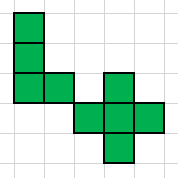
\includegraphics[height=1.25in]{good_move.png}}
  \hspace*{.2in}
  \raisebox{-0.25\height}{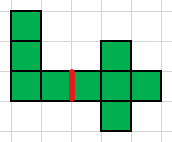
\includegraphics[height=1in]{bad_move.png}}
\end{minipage}
    \label{fig:moves}
\caption{Blokus configurations. Valid move (left) and invalid move (right)}
\end{figure}

\subsection{DQN Algorithms}

Deep Q-Learning (DQN) method \cite{dqn} was brought to solve many reinforcement learning issues. Multiple work have been done subsequently to improve DQN's efficiency on different tasks and environments.

This paper focuses on the Rainbow algorithm which combines:
\begin{itemize}
\item DQN
\item Double DQN (DDQN)
\item Prioritized Experience Replay (PER)
\item Dueling network
\item Categorical DQN
\item Noisy DQN
\item N-steps learning
\end{itemize}

\section{Methodology}

This section details how the action and observation spaces are organized over multiple environments and how the model is constructed.

\subsection{Observation and Action Spaces}

For this task, 9 Open AI \footnote{\url{https://openai.com/}} Gym Environments \footnote{\url{https://gym.openai.com/docs/}} consisting of three different boards were created:
\begin{itemize}
\item Simple: a smaller representation of the game for faster training time. This board is only for two players and all 5 tiles pieces from the original have been removed. This environment was used as a proof of concept.
\item Duo: the official Blokus duo game.
\item Hard: the official and original Blokus game.
\end{itemize}

The three boards can be used jointly with three different bots: 
\begin{itemize}
\item Random: selects randomly between all the possible moves.
\item Greedy: maximizes the number of tiles and then the number of newly blocked and opened corners.
\item Minimax: uses the same heuristic as greedy with 1 recursive call, which means trying to maximize the score looking one turn ahead.
\end{itemize}

The greedy player and the minimax player will try to optimize this function:
\begin{equation}
\begin{array}{l}
W_1 \times \textit{number of tiles} + \\
W_2 \times (\textit{available player's corners} - \textit{blocked opponent's corners})
\end{array}
\label{formula:score}
\end{equation}

The representation of the various boards available are shown in figures 1, 2 and 3.
\begin{table}[H]
\centering
\begin{tabular}{llll}
\hline
 & Simple & Duo & Hard \\
\hline
Board Size & $7\times7$ & $14\times14$ & $21\times21$ \\
Players & 2 & 2 & 4 \\
Observations & 147 & 588 & 2205 \\
Pieces & 12 & 21 & 21 \\
Actions & 919 & 13 729 & 33 854 \\
Average actions per turn & 19 & 160 & 200 \\
\hline
\end{tabular}
\caption{Characteristics per board type}
\label{tab:boards}
\end{table}

\begin{figure}[h!]
\centering
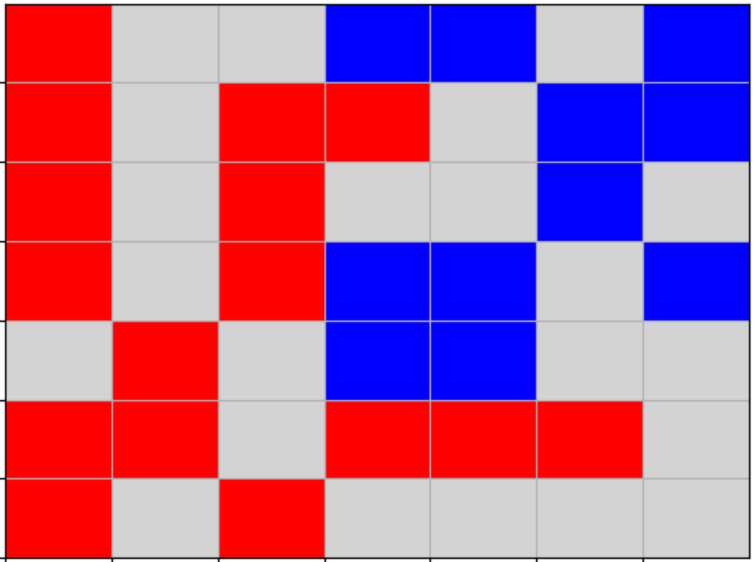
\includegraphics[height=2in]{simple_game.png}
\caption{The simple board}
  \label{fig:simpleBoard}
\end{figure}

\begin{figure}[h!]
\centering
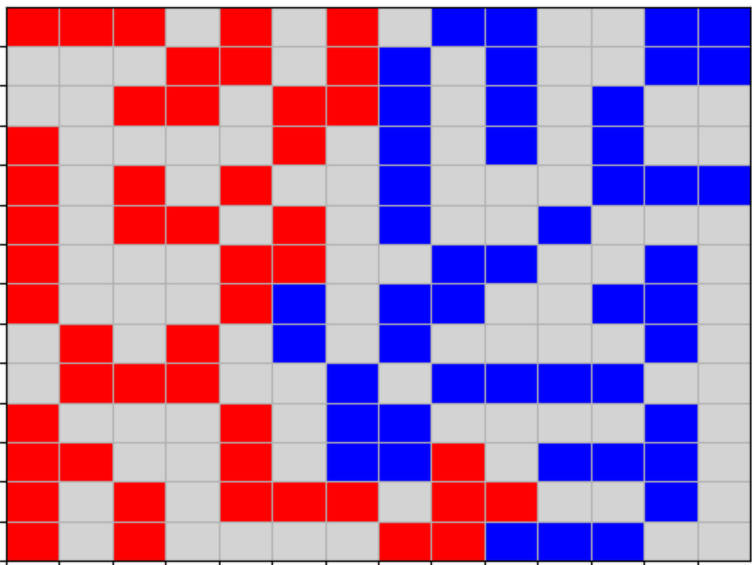
\includegraphics[height=2in]{duo_game.png}
  \caption{The duo board}
  \label{fig:duoBoard}
\end{figure}

\begin{figure}[h!]
\centering
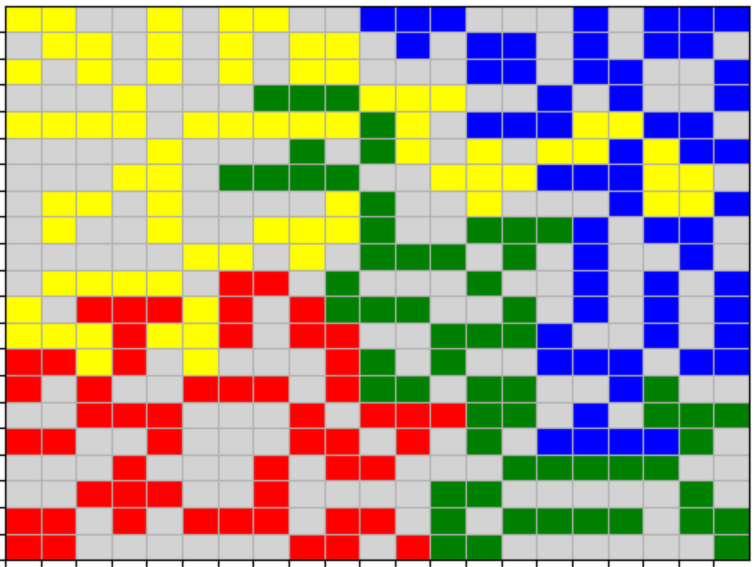
\includegraphics[height=2in]{hard_game.png}
  \caption{The hard board}
  \label{fig:hardBoard}
\end{figure}

\begin{align}
\textit{Observations} = \textit{Board Size} \times (\textit{Players} + 1)
\label{formula:observation}
\end{align}

The number of possible moves were calculated with the number of orientation and positions available on a given board. Each piece has 4 rotations (0, 90, 180 and 270 degrees) combined with a flip (either horizontal or vertical). Then, it can be placed on all the available translations on the board. The average actions per turn measures the mean number of available moves per turn. The reinforcement learning agent tries to take the best out of this number per turn. These results come from 100 simulations ran with a random agent.
 
\begin{figure}[h!]
\centering
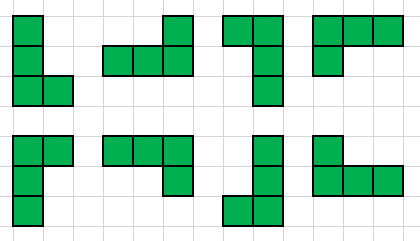
\includegraphics[height=1.5in]{8_moves.png}
  \caption{8 possible placements of the L4 piece}
  \label{fig:8moves}
\end{figure}

\begin{figure}[h!]
\centering
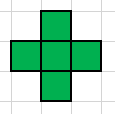
\includegraphics[height=0.75in]{single_move.png}
  \caption{Single possible placement of the X5 piece}
  \label{fig:singleMove}
\end{figure}

Finally, the rewards go as follow:
\begin{itemize}
\item +1 for a win
\item -1 for a lost
\item 0 for a tie
\item 0 for any other move
\end{itemize}

The environments are available for download on PyPi \footnote{\url{https://pypi.org/project/blokus-gym/}}. All the experiments and source code are available on GitHub \footnote{\url{https://github.com/frankilepro/blokus_ai}}.

\subsection{Rainbow Model}
Rainbow architecture \cite{rainbow} consisting of 6 different improvements of DQN was implemented to train the agent. Double DQN \cite{ddqn}, noisy network \cite{noisy}, prioritized experience replay \cite{per}, dueling architecture \cite{dueling}, n-steps learning \cite{nsteps} and categorical DQN were implemented separately and compared to regular DQN and Rainbow architecture. The value of the parameters used for training are presented in Table \ref{tab:rainbowparams}.

\begin{table}[H]
\centering
\begin{tabular}{ll}
\hline
 Parameters & Value \\
\hline
Number of episodes & 5000 \\
Learning rate & 0.001 \\
Batch size & 32 \\
N-steps & 3 \\
Gamma & 0.99 \\
Alpha (PER) & 0.6 \\
Beta (PER) & 0.6 \\
Number of atoms (Categorical) & 51 \\
\hline
\end{tabular}
\caption{Rainbow Training Parameters}
\label{tab:rainbowparams}
\end{table}

The input of the model is the state, which is represented by an n $\times$ n flattened matrix where n is the width of the board. Each player has an number from 1 to 4 attributed to represent their tiles. The output of the model represents the value of each actions. To ensure the agent only selects valid moves, an extra custom layer was added at the end of the network to filter only the possible moves. Invalid moves were attributed a value of $-\infty$. This way these actions are never chosen by the agent.

\section{Results}

The Blokus agent was trained on the 7 $\times$ 7 board against the random and the greedy player. Due to extensive training times, the AI agent was not trained on larger boards nor against the minimax player. On the Blokus game, Rainbow showed the best results and the fastest training (Figure \ref{fig:trainingRandom}). The average score used in Figure \ref{fig:trainingRandom} represents the average reward accumulated during training, thus can range from -1 to 1. Rainbow compared to DQN or single improvements of DQN performed significantly better. Prioritized experience replay (PER) and categorical DQN alone did not improve DQN's performance. However, combined with other Rainbow's improvements, PER and categorical had a positive impact on training (Figure \ref{fig:trainingRandom}). Unexpectedly, Rainbow without n-steps learning demonstrates a lower average score than DQN when trained on Blokus.

The Rainbow agent was put to the test against the random player, the greedy player and the minimax player (Table \ref{tab:gameresults}). It was trained against the greedy player, since minimax is exhaustively slow and time was limited. The agent obtained 69.8\% victory against the random player, 83.2\% victory against the greedy player and no victory against minimax. Rainbow tied minimax 43.8\% of the time. On average, the reinforcement agent beat a greedy and a random player, but could, at best, tie the minimax player.

\begin{figure}[H]
\centering
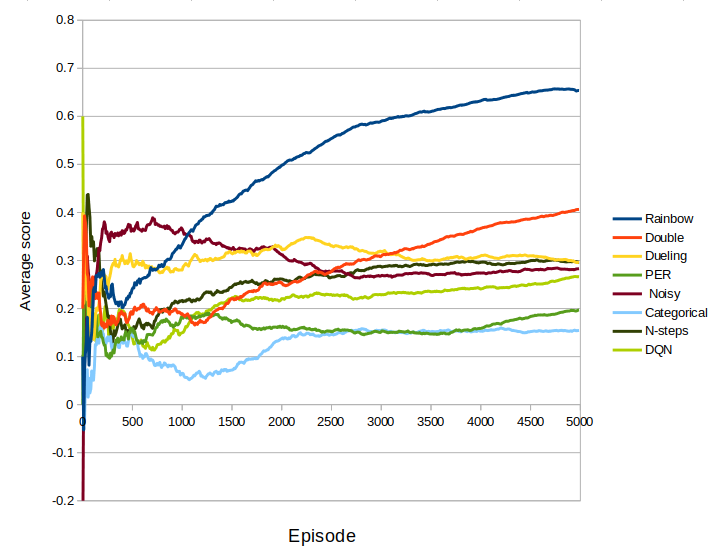
\includegraphics[height=2.5in, width=3in]{training_random.png}

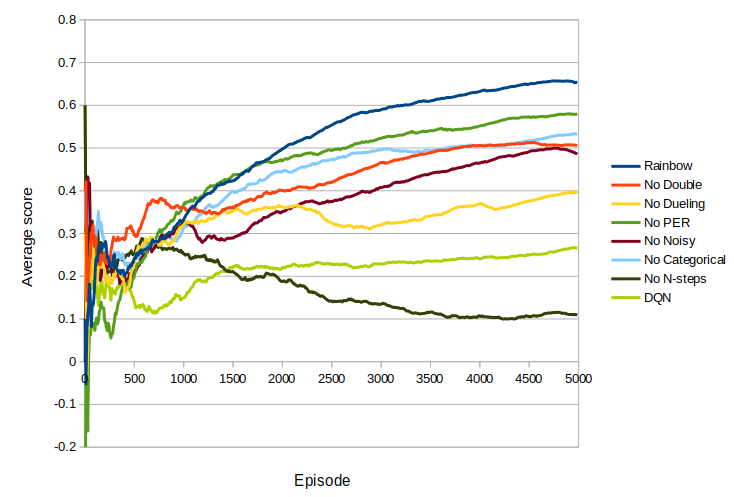
\includegraphics[height=2.5in, width=3in]{training_random_no.png}
\caption{Training Blokus Agent on Random Player}
\label{fig:trainingRandom}
\end{figure}

\begin{table}[H]
\centering
\begin{tabular}{llll}
\hline
 Player & Victories & Ties & Defeats \\
\hline
Random & 698 & 116 & 186 \\
Greedy & 832 & 81 & 87 \\
Minimax & 0 & 438 & 562 \\
\hline
\end{tabular}
\caption{Game results of Rainbow agent against different algorithm. The agent was trained against the greedy player.}
\label{tab:gameresults}
\end{table}

\section{Analysis}
The results obtained tend towards the ones presented in the original paper \cite{rainbow}. The Rainbow results are reproducible and adaptable to different tasks. Rainbow algorithm proved to be suited for learning and improving with the game of Blokus. The agent was able to beat a random and a greedy player in addition to tie a minimax bot.

On the other hand, the results could have been improved if more time was allowed to training and if the model had been exposed to different bot types during its training. Minimax, Duo and Hard environments were not used for training, but could have benefited the agent. Minimal manual optimization of hyper-parameters was performed. As showed in the previous section, the agents were only trained on either a greedy or random player. Even though the minimax agent was implemented, its extensive run time represented an obstacle during training. The time complexity is a result of the large action space which increases with each recursive call. Looking one or multiple turns ahead with the minimax agent is time consuming, even when fully multi-threaded, which limited its exploitation in this work. Alternatively, the opponent could have been chosen randomly with different probability distribution allowing in the process a broader variety of scenarios. Since the agent was trained only on a greedy bot and never on minimax, the results presented in table \ref{tab:gameresults} are expected. The agent was still able to tie about half the games with minimax. Rainbow agent wins more often against the greedy agent compared to the random agent, because the agent was trained on a greedy agent. Another hypothesis explaining the better performance of the agent on a greedy player is that the greedy agent is more predictable than a chaotic random player. Therefore, the Rainbow agent is more adapted to the greedy behaviour and does not have an optimal policy when faced against a random player.
 
Furthermore, the project in its current state, lacks the ability to train the model against itself. There are currently no automated mechanism to optimize the hyper-parameters of the model. These improvements could drastically improve the performance against stronger opponents. Finally, it could be interesting to have a mechanism allowing human players to play against any agents.

\section{Conclusion}
In the current work, we created a Blokus Gym environment, separated in 9 possible boards and player types. The Rainbow model \cite{rainbow} was reproduced by implementing separately 6 different DQN improvements. The RL agent was then trained on two of the Blokus environments. The results showed that the Rainbow agent had superior performance compared to DQN and other combinations of the DQN enhancements. When tested against a random, a greedy and a minimax player, the agent won most of the time against the random and the greedy bot, but couldn't defeat minimax. Training the agent on more challenging players and optimize the hyper-parameters of the model are changes that could improve the results. The larger boards created, Duo and Hard, should be tested in further work. It would also be interesting to a human player option to challenge the agent.


%% The file named.bst is a bibliography style file for BibTeX 0.99c
\bibliographystyle{named}
\bibliography{ijcai19}

\end{document}



